%%%%%%%%%%%%%%%%%%%%%%%%%%%%%%%%%%%%%%%%%%%%%%%%%%%%%%%
% Math 3250 Combinatorics, University of Connecticut
% Homework 1: A simple example for how to use LaTeX.
%%%%%%%%%%%%%%%%%%%%%%%%%%%%%%%%%%%%%%%%%%%%%%%%%%%%%%%

% Due date: Friday, January 25, 2019.

% Anything after a percent sign is a comment.

% Necessary first line. \documentclass defines the type of document and some options (for example, try changing 12pt to 10pt.
\documentclass[12pt]{amsart}

\usepackage{graphicx} % for including graphics

% The part of the tex file between the \documentclass
% and \begin{document} line is called the preamble.  
% Things having to do with setting up the document are done
% in the preamble.  You will not need to mess with it for now, except to change your name or the title your documents like I've done below. 
% After adding your name next to author, head down to where it says "Start here"

\title{Math 3250 Combinatorics Survey and \LaTeX \ Practice}
\author{Replace this text with your preferred first name and your last name}

\begin{document}

\maketitle

% --------------------------------------------------------
%                         Start here
% --------------------------------------------------------

This document is a beginning of the semester survey done in \LaTeX \ so that I can get to know you and you can practice with \LaTeX.  \ My comments in the source code (in blue) should help you with the \LaTeX \ commands.

% The following is an example for how to create an enumerated list: \begin{enumerate}\item first \item second \end{enumerate}
\begin{enumerate}
\item What is your home town? 
%name in emphasized/italics using \emph{ name of town }

\item What did you share about yourself on the first day of class?  What are some favorite sports or activities that you are involved in at UConn?
%in bold face using {\bf name of group } 

\item What is your favorite (math or otherwise) class in college so far?
% in bold face using  \textbf{name of favorite class}

\item What are some of your goals (academic or otherwise) for this semester?\\
REPLACE WITH YOUR GOALS
% To do a line break, use two negative-slope slashes as I demonstrated above 

\item What are some of your goals for after college? 
% Practice emphasizing just one word using \emph{ something to emphasize }

\item What do you hope to get out of this class? Why are you taking this class?
% This is how you create an itemized list (with bullet points)
\begin{itemize}
\item  Replace this text with your answer to the first question
\item  Replace this text your answer to the  second question
\end{itemize}

\item Please list all college-level in math/CS/stats/logic/philosophy, etc which you have successfully completed in the past 3 years:
\begin{enumerate}
\item replace this text with a class
\item replace this text with another class
\item replace this text with another class
% to add another item to this list, just write  \item
\end{enumerate}

\item If 
\[ f(x) = x^3 + e^x \]
then the derivative of $f$ is $\dots$ 
%  \[ put some math symbols here \]
% note how exponents are given using the carrot symbol ^

\item \label{itm:a_sequence} A sequence is defined by
\[ x_n = \frac{n}{n^2+1}. \]
What is a formula for $x_{n+1}$?
% note how subscripts are given using the underscore _.
%  note how you can also use dollar signs for math symbols: $put your math symbols between two dollar signs$

\item Using the sequence in problem (\ref{itm:a_sequence}), what is 
  \[ \lim_{n \to \infty} x_n? \]
% note how the stuff below the lim is enclosed in brackets.
% What does \to print?

\item What Greek letters are used in the definition of the limit?
(How about epsilon and delta, but I want you to typeset them. For example, to write the Greek letters alpha and beta, you would simply type $\alpha$ and $\beta$. If you wish, you can look up and practice writing your favorite Greek letters.) 


\item A permutation $f$ of the set $\{1,2,3,\dots,n\}$ is defined as a bijection $f: \{1,2,3,\dots,n\} \to \{1,2,3,\dots,n\}$.
% Again, we practice using the command \to
% Please replace the letter f for the function above with a Greek letter.


\item Express $1+\frac{1}{2}+\left(\frac{1}{2}\right)^2 + \cdots$ using
  the summation notation. 
%\sum gives you the summation notation.  
% _ can be used for what you write below the summation notation
% ^ can be used to write above the summation notation.

\item Please look at the source code below for typesetting a matrix. Consider the matrices  
\[
R =
  \begin{bmatrix}
    -1 & 0 & 0 \\
    0 & \cos{\theta} & \sin{\theta} \\
    0 & \sin{\theta} & -\cos{\theta}
  \end{bmatrix}
~\text{ and }~
S = 
  \begin{bmatrix}
    -1 & 0 & 0 \\
    0 & 1 & 0 \\
    0 & 0 & 1
  \end{bmatrix}.
\]
Recall or google how to compute the \emph{determinant} of a $3 \times 3$ matrix, and compute $det(R)$ and $det(S)$.

\item Write below a $3 \times 3$ matrix (or larger) which has determinant $-1$.

\item 
We can easily attach a captioned figure to a \LaTeX document and cite the figure. For example, Figure \ref{fig:jonathan14} shows Jonathan XIV, posing for a portrait. In Figure \ref{fig:jonathan14_13}, we see two dogs, Jonathan XIV (in the foreground) and Jonathan XIII. 

Your tasks are to find a picture of a different Husky, upload the image file to this Overleaf project, create a captioned figure environment (following my source code examples below), and use the backslash label and backslash ref commands to label and cite this new figure (following my examples in the previous sentence). 

\begin{figure}
    \centering
    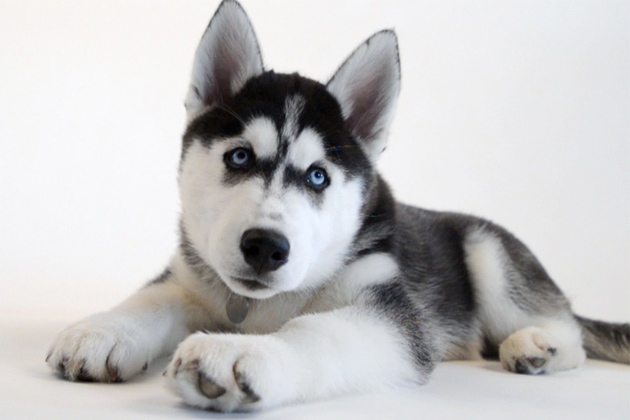
\includegraphics[height=5cm]{JonathanXIV.jpg}
    \caption{Jonathan XIV}
    \label{fig:jonathan14}
\end{figure}

\begin{figure}
    \centering
    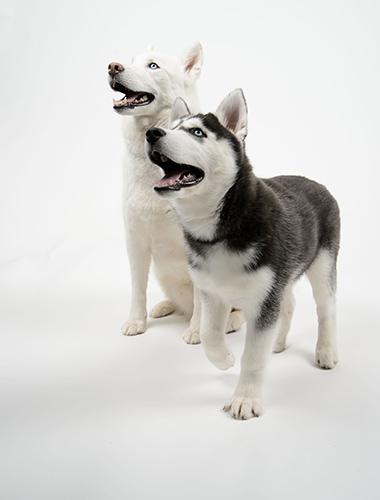
\includegraphics[height=5cm]{JonathanXIV_XIII.jpg}
    \caption{Jonathan XIV and Jonathan XIII}
    \label{fig:jonathan14_13}
\end{figure}
 
 
 
\item 
Imagine that you have written a book-length or article-length autobiography about your mathematical experiences. \emph{Write a passage, thought as a quote from your autobiography, that reveals something significant about you mathematically.} Please be as creative as you like. In case you are not feeling creative, here are a few suggested prompts: a story of your mathematical past; your current feelings about mathematics; 
positive and negative episodes from past math courses; moments in which math came up in other situations; plans for the future.\\
\underline{Note}: Your submission will be kept confidential, but you'll be asked to share a sentence with the rest of the class.
% Please write below

\item 
(optional) Is there anything else you'd like to tell me about yourself?

\end{enumerate}

\end{document}








